\newpage
\appendix
\section{Cinématique}

\begin{table}[H]
	\centering
	\caption{Valeurs des paramètres pour les cas d'études cinématiques}
	\label{tab:values-cinematique}
	\begin{tabular}{ll}
		\toprule
	  Variable & Valeur \\
		\midrule
		$l_0$ & 50 cm \\
		$l_1$ & 25 cm \\
		$l_2$ & 25 cm \\
		$\omega$ & 25 rad$/\textrm{s}^2$ \\
		\bottomrule
	\end{tabular}
\end{table}

\subsection{Mouvement horizontal}
\begin{figure}[H]
  \centering
	\begin{subfigure}{.45\linewidth}
		\centering
		\includegraphics[width=\textwidth]{figures/horizontal-pos.pdf}
		\caption{Position en $x$}
		\label{fig:horizontal-pos}
	\end{subfigure}
	\begin{subfigure}{.45\linewidth}
		\centering
		\includegraphics[width=\textwidth]{figures/horizontal-v.pdf}
		\caption{Vitesse en $x$}
		\label{fig:horizontal-v}
	\end{subfigure}

	\begin{subfigure}{.5\linewidth}
		\centering
		\includegraphics[width=\textwidth]{figures/horizontal-alpha.pdf}
		\caption{Accélération en $x$}
		\label{fig:horizontal-alpha}
	\end{subfigure}

	\caption{Attributs du point $A$ lorsqu'il est contraint à un mouvement horizontal}
	\label{fig:horizontal-plots}
\end{figure}

\begin{figure}[H]
  \centering
\begin{subfigure}{.26\linewidth}
		\centering
		\includegraphics[width=\textwidth]{figures/x-bound-fig-before.pdf}
		\caption{Lorsque $\theta=0$}
		\label{fig:horizontal-before}
	\end{subfigure}
	\hspace{1cm}
	\begin{subfigure}{.2\linewidth}
		\centering
		\includegraphics[width=\textwidth]{figures/x-bound-fig-after.pdf}
		\caption{Lorsque $\theta=\frac{\pi}{3}$}
		\label{fig:horizontal-after}
	\end{subfigure}
		\caption{Positionnement du bras contraint à un mouvement en $x$ selon $\theta$}
	\label{fig:horizontal-fig}
\end{figure}

\subsection{Mouvement vertical}

\begin{figure}[H]
  \centering
	\begin{subfigure}{.43\linewidth}
		\centering
		\includegraphics[width=\textwidth]{figures/vertical-pos.pdf}
		\caption{Position en $y$}
		\label{fig:vertical-pos}
	\end{subfigure}
	\begin{subfigure}{.43\linewidth}
		\centering
		\includegraphics[width=\textwidth]{figures/vertical-v.pdf}
		\caption{Vitesse en $y$}
		\label{fig:vertical-v}
	\end{subfigure}

	\caption{Attributs du point $A$ lorsqu'il est contraint à un mouvement vertical}
	\label{fig:vertical-plots}
\end{figure}

\begin{figure}[H]
  \centering
	\begin{subfigure}{.36\linewidth}
		\centering
		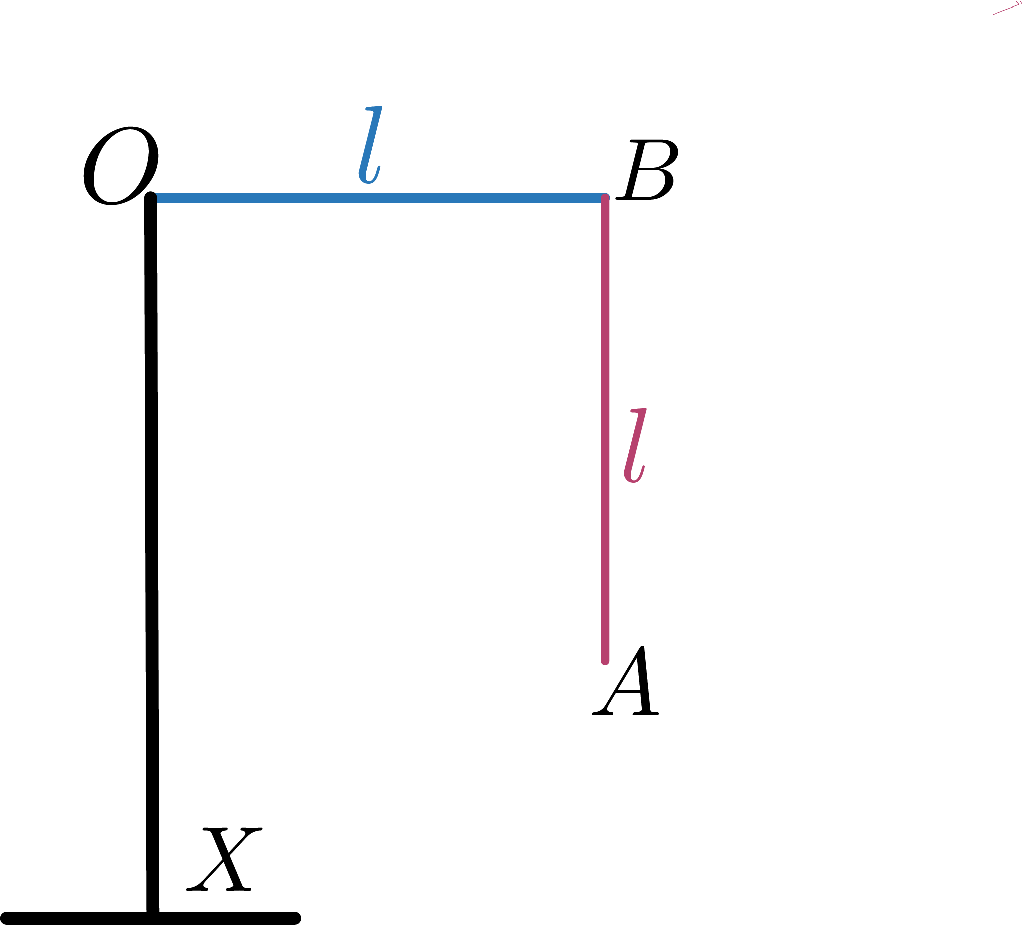
\includegraphics[width=\textwidth]{figures/vert-before.pdf}
		\caption{Lorsque $\theta=0$}
		\label{fig:vertical-before}
	\end{subfigure}
	\hspace{1cm}
	\begin{subfigure}{.3\linewidth}
		\centering
		\includegraphics[width=\textwidth]{figures/vert-after.pdf}
		\caption{Lorsque $\theta=\frac{\pi}{3}$}
		\label{fig:vertical-after}
	\end{subfigure}
		\caption{Positionnement du bras contraint à un mouvement en $y$ selon $\theta$}
	\label{fig:vertical-fig}
\end{figure}

\section{Simulations statiques et dynamiques}

\begin{table}[H]
	\centering
	\caption{Valeurs des paramètres pour les cas d'études statiques et dynamiques}
	\label{tab:values-statique-dynamique}
	\begin{tabular}{ll}
		\toprule
	  Variable & Valeur \\
		\midrule
		$l_0$ & 50 cm \\
		$l_1$ & 25 cm \\
		$l_2$ & 25 cm \\
		$m_A$ & 100 g \\
		$m_{BA}$ & 1 kg \\
		$\alpha_{BA}$ & 5 rad/s$^2$ \\
		\bottomrule
	\end{tabular}
\end{table}

\begin{figure}[H]
  \centering
  \includegraphics[width=0.7\textwidth]{figures/static-torque.pdf}
  \caption{Couple résultant $M_{B_z}$ en fonction de l'angle $\varphi$ (cas statique)}
  \label{fig:static-torque}
\end{figure}

\begin{figure}[H]
  \centering
  \includegraphics[width=0.7\textwidth]{figures/dynamic-torque.pdf}
  \caption{Couple résultant $M_{B_z}$ en fonction de l'angle $\varphi$ (cas dynamique avec $\ddot{\varphi} = 5$ rad/s$^2$)}
  \label{fig:dynamic-torque}
\end{figure}
